\documentclass[11pt]{article}

\usepackage{amssymb,amsmath,amsthm}
\usepackage{verbatim}
\usepackage{fullpage}
\usepackage{gencor}
\usepackage{mathrsfs}
\usepackage{authblk}
\usepackage{graphicx}
\usepackage{caption}
\usepackage{subcaption}
\usepackage{multirow}
\usepackage[nottoc,notlof,notlot,numbib]{tocbibind}
\usepackage{xr-hyper}
\externaldocument[supp-]{supp}
\makeatletter
\renewcommand*{\@fnsymbol}[1]{\ensuremath{\ifcase#1\or *\or**\or\dagger\or \ddagger\or
   \mathsection\or \mathparagraph\or \|\or **\or \dagger\dagger
   \or \ddagger\ddagger \else\@ctrerr\fi}}
 \newcommand{\beginsupplement}{%
        \setcounter{table}{0}
        \renewcommand{\thetable}{S\arabic{table}}%
        \setcounter{figure}{0}
        \renewcommand{\thefigure}{S\arabic{figure}}%
     }

\makeatother

\frenchspacing
\title{An Atlas of Genetic Correlations across Human Diseases and Traits}
\author[1,2,3]{Brendan Bulik-Sullivan$^{\dagger}$\thanks{Co-first authors}$^,$}
\author[*,4]{Hilary K Finucane}
\author[1,2,3]{Verneri Antilla}
\author[5,6]{Alexander Gusev}
\author[7]{Felix R. Day}
\author[8]{ReproGen Consortium}
\author[8]{Psychiatric Genomics Consortium}
\author[8]{Genetic Consortium for Anorexia Nervosa of the Wellcome Trust Case Control Consortium 3}
\author[7]{John R.B. Perry}
\author[1]{Nick Patterson}
\author[1,2,3]{Elise Robinson}
\author[1,2,3]{Mark J Daly}
\author[1,5,6]{Alkes L Price\thanks{Co-last authors}$^,$}
\author[**,1,2,3]{Benjamin M Neale\thanks{Correspondence should be addressed to BBS (bulik@broadinstitute.org) or BMN (bneale@broadinstitute.org).}}

\affil[1]{\small{Program in Medical and Population Genetics, Broad Institute of MIT and Harvard, Cambridge, MA, USA}}
\affil[2]{Stanley Center for Psychiatric Genetics, Broad Institute of MIT and Harvard, Cambridge, MA, USA}
\affil[3]{Analytic and Translational Genetics Unit, Massachusetts General Hospital and Harvard Medical School, Boston, Massachusetts, USA.}
\affil[4]{Department of Mathematics, Massachusetts Institute of Technology, Cambridge, MA, USA.}
\affil[5]{Department of Epidemiology, Harvard School of Public Health, Boston, MA, USA.}
\affil[6]{Department of Biostatistics, Harvard School of Public Health, Boston, MA, USA.}
\affil[7]{MRC Epidemiology Unit, University of Cambridge School of Clinical Medicine, Institute of Metabolic Science, Cambridge Biomedical Campus, Cambridge, CB2 0QQ, UK}
\affil[8]{A list of members and affiliations appears in the Supplementary Note.}
\date{}
\begin{document}
\maketitle

\begin{abstract}
A recent focus in statistical genetics has been combining genetic association results from multiple phenotypes in order understand the relationships among traits.
In this paper, 
we estimate 300 genetic correlations among 25 traits, totaling more than 1.5 million unique phenotype measurements.
To enable this analysis, we introduce a statistical method based on LD Score regression for estimating genetic correlation using only GWAS summary statistics.
Our results include a positive genetic correlation between anorexia nervosa and schizophrenia and a negative genetic correlation between anorexia nervosa and body mass index, as well as a large number of replications and positive controls. 
These results highlight the power of a polygenic modeling framework, since there currently are no genome-wide significant SNPs for anorexia nervosa. 
 
\end{abstract}
\newpage
%%%%%%%%%%%%%%%%%%%%%%%%%%%%%%%%%%%%%%%%%%%%%%%%%%%%%%%%%%%%%%%
\section*{Introduction}
\label{Introduction}
%%%%%%%%%%%%%%%%%%%%%%%%%%%%%%%%%%%%%%%%%%%%%%%%%%%%%%%%%%%%%%%

Discovering correlations between phenotypes is a fundamental goal of epidemiology, 
with applications to classification and treatment of disease, as well as to development of pharmaceutical drugs.  
One classical strategy in epidemiology is to search for correlations between phenotypes via cross-sectional or longitudinal observational studies; 
however, the interpretation of results from these studies can be confounded and are vulnerable to reverse causation  \cite{smith2003mendelian, smith2014mendelian}. 
An alternative strategy that is effective for heritable traits and is more robust to confounding is to search instead for pairs of phenotypes with shared genetic etiology. 

The earliest methods for searching for traits with genetic overlap were twin and family studies \cite{vandenberg1965multivariate, 
kempthorne1961interpretation,
loehlin1966genetic,
neale1992methodology,
lichtenstein2009common},
which have been applied to a wide spectrum of traits.
However, family methods have the disadvantage of requiring measurements of different traits on the same individuals.
Genome-wide association studies (GWAS) produce effect-size estimates for specific genetic variants, so it is possible to test for shared genetic
etiology using these effect-size estimates, circumventing the requirement to measure multiple traits per individual.
This can substantially reduce the cost and difficulty of epidemiological studies for uncommon diseases and traits that are expensive to assay.

One widely-used technique for testing relationships between phenotypes using GWAS data is Mendelian randomization  
\cite{smith2003mendelian, smith2014mendelian}, which is the specialization to genetics of instrumental variables \cite{angrist2008mostly}.
Mendelian randomization has proved effective for traits for which large-effect genetic variants have been identified \cite{voight2012plasma,do2013common};
however for many complex traits, the heritability is distributed over thousands of variants with small effects \cite{visscher2012five},
in which case Mendelian randomization using genome-wide significant SNPs suffers from low power and weak instrument bias \cite{angrist2008mostly}.

In this paper, our goal is to estimate genetic correlation, a quantity whose definition includes the effects of all SNPs, including those that do not reach genome-wide significance (Methods).
In cases where two phenotypes are suspected of having a cause-effect relationship,
genetic correlation can be interpreted as a re-scaling of the instrumental variables estimate obtained from an instrument constructed using all SNPs (Methods);
however, unlike instrumental variables, genetic correlation is also meaningful for pairs of diseases, and can be interpreted as a genetic analogue of comorbidity.
The two main existing techniques for estimating genetic correlation from GWAS data are restricted maximum likelihood (REML) \cite{yang2010, yang2011gcta, lee2012estimation, pgccdg2013, vattikuti2012heritability, chen2014estimation}
and polygenic scores \cite{purcell2009common, dudbridge2013power}.
These methods have only been applied to a small number of traits so far, 
because these methods require individual genotypes, 
which are often difficult to obtain due to privacy considerations and informed consent limitations. 

Here, we introduce a computationally fast method related to LD Score regression \cite{buliksullivan2014} for estimating genetic correlation that requires only GWAS summary statistics and is not biased by sample overlap.
We apply this method to data from 25 GWAS and report genetic correlations between 300 pairs of phenotypes. 

%%%%%%%%%%%%%%%%%%%%%%%%%%%%%%%%%%%%%%%%%%%%%%%%%%%%%%%%%%%%%%%
\section*{Results}\label{Results}
%%%%%%%%%%%%%%%%%%%%%%%%%%%%%%%%%%%%%%%%%%%%%%%%%%%%%%%%%%%%%%%

\subsection*{Overview of Methods}

Our method for estimating genetic correlation from summary statistics relies on the fact that the GWAS effect-size estimate for a given SNP incorporates the effects of all SNPs in LD with that SNP \cite{yang2011genomic,buliksullivan2014}. 
For a polygenic trait, SNPs in regions with strong LD will have higher $\chi^2$-statistics on average than SNPs in regions with little LD \cite{buliksullivan2014}. 
A similar relationship holds if we replace $\chi^2$-statistics for a single study with the product $z_{1j}z_{2j}$, 
where $z_{ij}$ denotes the $Z$-score for study $i$ and SNP $j$.

More precisely, under a polygenic model \cite{yang2010,lee2012estimation}, the expected value of $z_{1j}z_{2j}$ is 
\begin{equation}\label{reg_eqn}
	\E[z_{1j}z_{2j}] = \dfrac{\sqrt{N_1N_2}\rho_g}{M}\ell_j + \dfrac{\rho N_s}{\sqrt{N_1N_2}},
\end{equation}
where $N_i$ is the sample size for study $i$, $\rho_g$ is genetic covariance (defined in Methods), $\ell_j$ is LD Score \cite{buliksullivan2014}, $N_s$ is the number of samples shared between study 1 and study 2, and $\rho$ is the phenotypic correlation among the $N_s$ overlapping samples (Supplementary Note).
If study 1 and study 2 are the same study, then this reduces to the single-phenotype result from \cite{buliksullivan2014}, because the genetic covariance between a trait and itself is the same as heritability, and $\chi^2 = z^2$.
As a consequence of equation 1, we can estimate genetic covariance using the slope from the regression of $z_{1j}z_{2j}$ on LD Score, which is computationally very fast (see Methods). 
If we normalize genetic covariance to lie in the interval $[-1,1]$, we obtain genetic correlation: 
$r_g := \rho_g/\sqrt{h^2_1h^2_2},$ where $h^2_i$ denotes the SNP-heritability from study $i$. 
Theory and extensive simulations confirm that our method produces robust estimates of genetic correlation, even when summary statistics are affected by population stratification \cite{buliksullivan2014} or sample overlap (Supplementary Note).

\subsection*{Replication of PGC Cross Disorder Results}\label{PGCCDG}

For validation, we replicated the estimates of genetic correlations between psychiatric disorders obtained with
individual genotypes and REML by the Psychiatric Genomics Consortium (PGC) \cite{pgccdg2013}, 
using LD Score regression and summary statistics from the same data \cite{cross2013identification}.
Since the summary statistics from \cite{cross2013identification} used non-overlapping samples, 
we also estimated genetic correlation using LD Score regression with constrained intercept (Methods).
Results from this analysis are displayed in Figure \ref{Fig:Replication of PGC Cross-Disorder Results}.
As expected, the genetic correlation estimates from LD Score regression were similar to the results from REML.
LD Score regression without intercept gave standard errors that were only slightly larger than REML,
while the standard errors from LD Score regression with intercept were larger, especially for traits with small sample sizes
(\emph{e.g.,} ADD, ASD).


% Figure 1 -- replication of PGC-CDG results
\begin{figure}[!ht]
\begin{centering}
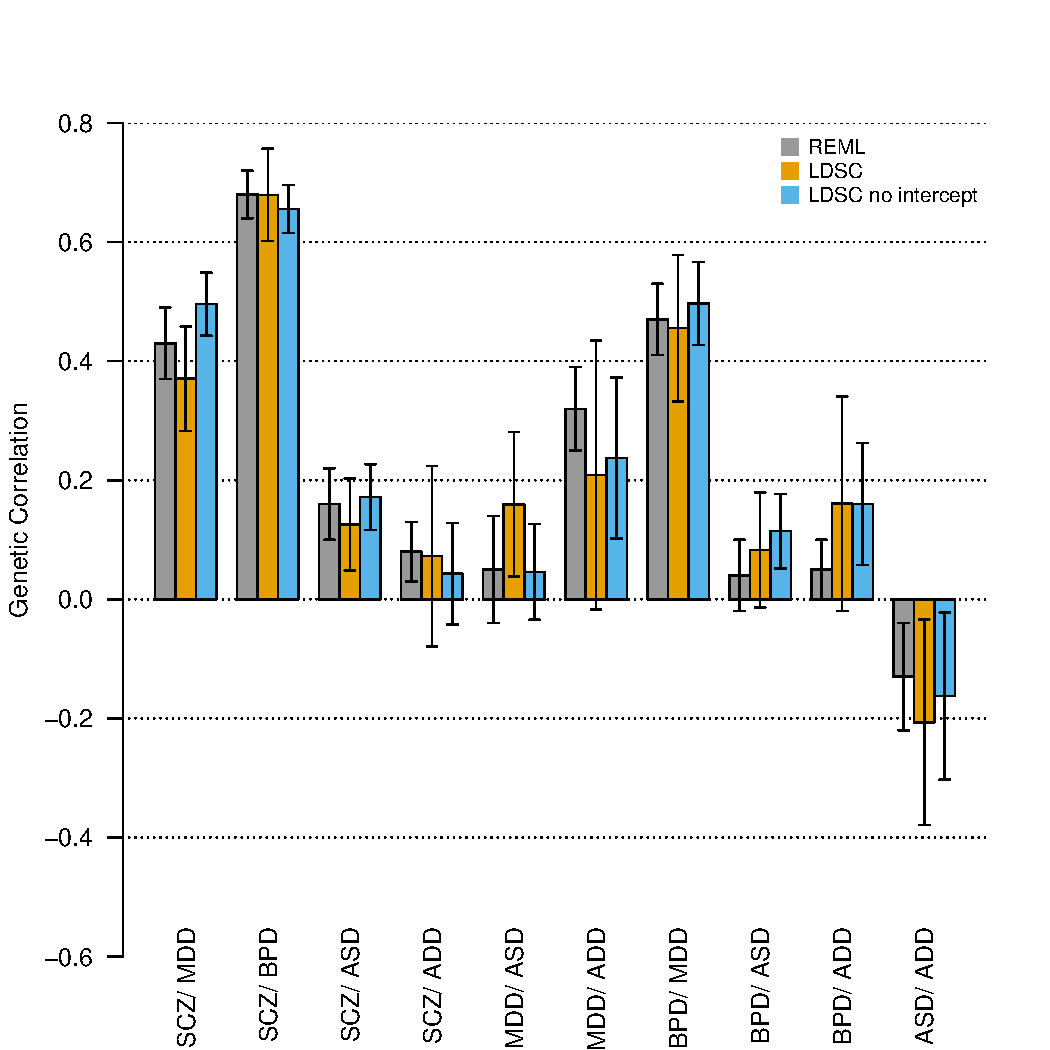
\includegraphics[scale=0.9]{figs/ldsc_vs_gcta.pdf}
\end{centering}
\caption{\label{Fig:Replication of PGC Cross-Disorder Results}\small{\textit{Replication of PGC Cross-Disorder Results.
This plot compares LD Score regression estimates of genetic correlation using the summary statistics from \cite{cross2013identification} (which were generated from approximately the same data as \cite{pgccdg2013}) to 
estimates obtained from REML in \cite{pgccdg2013}.
The horizontal axis indicates pairs of phenotypes, and the vertical axis indicates genetic correlation.
The error bars show standard errors.
Colors indicate different estimation procedures. Green is REML,
orange is LD Score with intercept and white is LD Score with constrained intercept.
The estimates of genetic correlation between psychiatric phenotypes in figure \ref{Fig:300 Gencors} use larger sample sizes;
this plot is intended primarily as a technical validation.
Abbreviations: 
ADD = attention deficit hyperactivity disorder;
ASD = autism spectrum disorder;
BPD = bipolar disorder;
MDD = major depressive disorder;
SCZ = schizophrenia.}}}
\end{figure}

\subsection*{Application to Summary Statistics From 25 Phenotypes}

We used LD Score regression to estimate genetic correlations among 25 phenotypes (URLs, Methods).
Genetic correlation estimates for all 300 pairwise combinations of the 25 traits are displayed in Figure \ref{Fig:300 Gencors}.
For clarity of presentation in this figure, 
we pruned to one phenotype from each cluster of highly correlated phenotypes (Methods).
Highly correlated anthropometric, smoking, and insulin-related phenotypes that were excluded from Figure \ref{Fig:300 Gencors}
are displayed in Tables \ref{giant}, \ref{smoking} and \ref{insulin}, respectively.
The genetic correlation between the two educational attainment phenotypes -- years of education and college (yes/no) -- studied by Rietveld \emph{et al.} \cite{rietveld2013gwas} was 100\%, so we present the genetic correlation results for the college phenotype only.

% Figure 2 -- Genetic correlation heatmap with 25 traits
\begin{figure}[!ht]
\begin{centering}
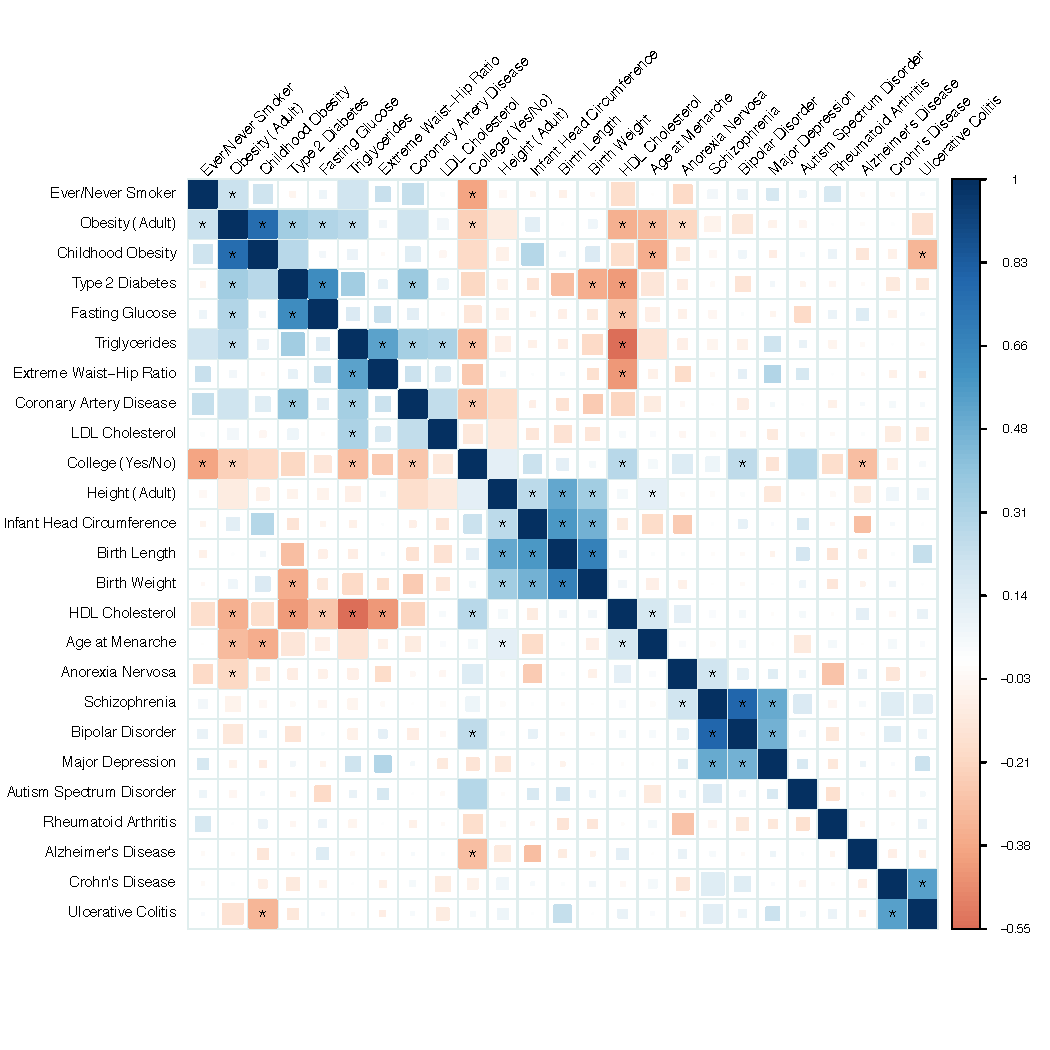
\includegraphics[scale=0.9]{figs/rg_heatmap.pdf}

\caption{         
\label{Fig:300 Gencors}
\small{\textit{Genetic Correlations among 25 Published GWAS.
Blue corresponds to positive genetic correlations; red corresponds to negative genetic correlation. 
Larger squares correspond to more significant $p$-values.
Genetic correlations that are different from zero at 1\% FDR are displayed as full-sized squares. 
Genetic correlations that are significantly different from zero at significance level 0.05 after Bonferroni correction for the 300 tests in this figure are given an asterisk. 
We display results that do not pass multiple testing correction as smaller squares in order to avoid the confusion that would result from whiting our positive controls that do not pass multiple testing correction because of small sample size.
This multiple testing correction is conservative, since the tests are not independent.
}}}
\end{centering}
\end{figure}

% Results that are consistent with top SNP results or MR analyses 
For the majority of pairs of traits in Figure \ref{Fig:300 Gencors}, no GWAS-based genetic correlation estimate has been reported; 
however, many associations have been described in an \emph{ad-hoc} manner based off the observation of overlap among genome-wide significant loci.
Examples of genetic correlations that are consistent with overlap among top loci include the correlations between plasma lipids and cardiovascular disease \cite{do2013common}; age at onset of menarche and obesity \cite{perry2014parent}; type 2 diabetes, obesity, fasting glucose, plasma lipids and cardiovascular disease \cite{morris2012large}; birth weight, adult height and type 2 diabetes \cite{horikoshi2013new}; birth length, adult height and infant head circumference \cite{early2012genome, taal2012common}; and childhood obesity and adult obesity \cite{early2012genome}. 
For many of these pairs of traits, we can reject the null hypothesis of zero genetic correlation with overwhelming statistical
significance (\emph{e.g.,} $p=6\times10^{-24}$ for age at onset of menarche and obesity; $p=6\times10^{-52}$ for obesity and childhood obesity).

% Table 1 -- interesting genetic correlation results highlighted in the main text
\begin{table}[h!]
\centering
\begin{tabular}{ l|llll}
 & Phenotype 1 & Phenotype 2 & $r_g$ (se) & $p$-value \\
\hline
\multirow{13}{*}{Epidemiological} 
& Age at Menarche & Height (Adult) & 0.11 (0.03) & $6\times10^{-5\ **}$  \\
& Age at Menarche & Type 2 Diabetes & -0.13 (0.04) & $3\times10^{-3}$  \\
& Age at Menarche & Triglycerides & -0.15 (0.04) & $1\times10^{-3\ *}$ \\
& Coronary Artery Disease & Age at Menarche &  -0.11 (0.05) & $4\times10^{-2}$ \\
& Coronary Artery Disease & College (Yes/No) & -0.278 (0.07) & $1\times10^{-4\ **}$ \\
& Coronary Artery Disease & Height (Adult) &  -0.17 (0.05) & $2\times10^{-4\ *}$\\
& Alzheimer's & College (Yes/No) & -0.30 (0.08) & $1\times10^{-4\ **}$ \\
& Bipolar Disorder & College (Yes/No) & 0.026 (0.064) & $6\times10^{-5\ **}$ \\
& Obesity (Adult) & College (Yes/No) & -0.23 (0.04) & $2\times10^{-8\ **}$\\
& Triglycerides & College (Yes/No) &-0.30 (0.04)&$5\times10^{-12\ **}$ \\
& Anorexia Nervosa & Obesity (Adult) & -0.20 (0.04) & $4\times10^{-6\ **}$ \\
& Ever/Never Smoker & College (Yes/No) & -0.39 (0.07) & $1\times10^{-9\ **}$ \\
& Ever/Never Smoker & Obesity (Adult) & 0.22 (0.05) & $7\times10^{-5\ **}$ \\
\hline
\multirow{3}{*}{Novel/Nonzero} 
& Autism Spectrum Disorder & College (Yes/No) & 0.28 (0.08) & $5\times10^{-4\ *}$\\
& Ulcerative Colitis & Childhood Obesity & -0.33 (0.08) & $3.9\times10^{-5\ **}$\\
& Anorexia Nervosa & Schizophrenia & 0.19 (0.04)  & $1.5\times10^{-5\ **}$ \\
\hline
\multirow{8}{*}{Novel/Zero} 
& Schizophrenia &Alzheimer's &  0.05 (0.05) & 0.58 \\
& Schizophrenia & Ever/Never Smoker & 0.03 (0.06) & 0.26 \\
& Schizophrenia & Triglycerides & -0.05 (0.04) & 0.21 \\
& Schizophrenia & LDL Cholesterol & -0.02 (0.03) & 0.64 \\
& Schizophrenia & HDL Cholesterol & 0.03 (0.04) & 0.50 \\
& Schizophrenia & Rheumatoid Arthritis & -0.05 (0.05) & 0.38 \\
& Crohn's Disease & Rheumatoid Arthritis & -0.02 (0.09) & 0.83 \\
& Ulcerative Colitis & Rheumatoid Arthritis & -0.09 (0.09) & 0.33 \\
\end{tabular}
\caption{
\small{\textit{\label{table:results}Genetic correlation estimates, standard errors and $p$-values for selected pairs of traits. Results are grouped into
 genetic correlations that are novel genetic results, but are consistent with established epidemiological associations (``Epidemiological''), novel genetic correlations (``Novel/Nonzero'') and interesting null results (``Novel/Zero''). 
 The $p$-values displayed are uncorrected $p$-values.
Results that pass multiple testing correction for the 300 tests in Figure \ref{Fig:300 Gencors} at 1\% FDR are given a single asterisk; results that pass Bonferroni correction at significance level 0.05 are given two asterisks.
For completeness, we present some genetic correlations that are directionally consistent with epidemiological associations but that do not pass multiple testing correction in our data. }}}
\end{table}

% Novel genetic results that are not novel epidemiological results
The first section of table \ref{table:results} lists genetic correlation results that are consistent with well-known epidemiological associations, 
but, as far as we are aware, have not previously been reported using genetic data.
Our estimates of the genetic correlation between age at onset of menarche and adult height \cite{onland2005age}, cardiovascular disease \cite{day2014} and type 2 diabetes \cite{day2014, elks2013age} are consistent with the epidemiological associations. 
Our estimate of a negative genetic correlation between AN and obesity (and a similar genetic correlation with BMI) is intriguing given that the most striking feature of anorexia nervosa is the ability to maintain dangerously low BMI \cite{american2013dsm} and suggests that similar genetic factors may influence normal variation in BMI as well as severely dysregulated BMI in psychiatric illness.
This result is consistent with our observation that BMI GWAS findings appear to primarily implicate neuronal, rather than metabolic, cell-types and epigenetic marks 
\cite{finucane2014partitioning}.
The negative genetic correlation between adult height and coronary artery disease agrees with a replicated epidemiological association  \cite{wang2011associations,hebert1993height,rich1995height}.
We observe several significant associations with the educational attainment phenotypes from
Rietveld \emph{et al.} \cite{rietveld2013gwas}.
We estimate a statistically significant negative genetic correlation between college and Alzheimer's disease, 
consistent with the epidemiological observation that low educational attainment is one of the largest risk factors for Alzheimer's
\cite{barnes2011projected, norton2014potential}. 
The positive genetic correlation between college and bipolar disorder is consistent with psychiatric literature showing that educational attainment and bipolar disorder status are positively correlated
\cite{maccabe2010excellent, tiihonen2005premorbid}, 
Our estimate of a negative genetic correlation between smoking and college is consistent with the epidemiological result that smoking is more prevalent among less-educated groups \cite{pierce1989trends}.

% Novel results
The second section of table \ref{table:results} lists results that are, to the best of our knowledge, new both to genetics and epidemiology.
First, we find a positive genetic correlation between between anorexia nervosa and schizophrenia.
Comorbidity between eating and psychotic disorders has not been thoroughly investigated in the psychiatric literature \cite{striegel1999psychiatric,blinder2006psychiatric}, and our results raise the intriguing possibility of fundamental similarity between these classes of disease.
Second, we estimate a negative genetic correlation between ulcerative colitis and childhood obesity.
The relationship between premorbid BMI and ulcerative colitis is at present not well-understood,
and our results suggest that exploring this relationship may be a fruitful direction for further investigation. 
Third, we estimate a positive genetic correlation between autism spectrum disorder (ASD) and educational attainment,
which itself has very high genetic correlation with IQ \cite{deary2007intelligence, calvin2010sex, rietveld2013gwas}.
The ASD summary statistics were generated using a case-pseudocontrol study design, so this result cannot be explained by diagnostic biases, such as the tendency for the parents of children who receive a diagnosis of ASD to be better educated than the general population \cite{durkin2010socioeconomic}. 
The distribution of IQ among individuals with ASD has lower mean than the general population, but with heavy tails \cite{robinson2014autism} (\emph{i.e.,} an excess of individuals with extremely low and extremely high IQ).
In addition, there is evidence that the genetic architectures of high IQ and low IQ ASD are dissimilar \cite{samocha2014framework}.
We are unable to offer an explanation for this result, but propose that further exploration of this genetic correlation is an interesting direction for future research.

% Interesting null results
Next, the third section of table \ref{table:results} lists several instances where the genetic correlation is close to zero with small standard error, in contrast to previous reports of epidemiological correlation or pleiotropy.
We estimate genetic correlations close to zero between schizophrenia and rheumatoid arthritis, schizophrenia and smoking, and schizophrenia and plasma lipids. The lack of genetic correlation between schizophrenia and rheumatoid arthritis is interesting because schizophrenia has been observed to be protective for rheumatoid arthritis \cite{silman2002epidemiology}.
The absence of genetic correlation between schizophrenia and smoking is notable because of the high prevalence of smoking among individuals with schizophrenia \cite{de2005meta}. 
Our estimate of zero genetic correlation between schizophrenia and plasma lipid levels or cardiovascular disease contrasts with earlier reports of extensive pleiotropy between schizophrenia and triglycerides \cite{andreassen2013improved2}. 
However, the observation from Andreassen, \emph{et al.} \cite{andreassen2013improved2} could potentially be explained the sensitivity of the method used in the original report to the properties of a few regions with high linkage disequilibrium, 
rather than trait biology (Table \ref{qq_tg}).
We estimate near-zero genetic correlation between Alzheimer's disease and schizophrenia. 
The genetic correlations between the other four psychiatric traits (anorexia nervosa, bipolar, major depression, ASD) are also
close to zero, but with larger standard errors, due to smaller sample sizes.
This suggests that the genetic basis of Alzheimer's disease is distinct from psychiatric conditions. 
Last, we estimate near zero genetic correlation between rheumatoid arthritis and both Crohn's disease and ulcerative colitis. Although these immune diseases share a large number of associated loci \cite{cotsapas2011pervasive,farh2014genetic}, 
it is as often the case that an allele that is risk-increasing for one immune disease is protective for another as an allele is 
risk-increasing for two \cite{cotsapas2011pervasive}, consistent near-zero genetic correlation overall.
This is an example of pleiotropy without genetic correlation (Methods).
%%% Getting # of overlapping gwsig loci w/ concordant and discordant effects from Mark D

% Results that are consistent with previously reported GWAS rg's (moved this from the beginning of the results section to the end in order to present more interesting results first
Finally, our estimates of genetic correlations among metabolic traits are consistent with the estimates obtained using REML in Vattikuti \emph{et al.}
\cite{vattikuti2012heritability} (Supplementary Table \ref{supp-vattikuti}), and are directionally consistent with the recent Mendelian randomization results from Wuertz \emph{et al.} \cite{wuertz2014metabolic}.
In addition, our estimate of 0.57 (0.074) for the genetic correlation between Crohn's disease and ulcerative colitis is consistent
with the estimate of 0.62 (0.042) from Chen \emph{et al.} \cite{chen2014estimation}.
 


%%%%%%%%%%%%%%%%%%%%%%%%%%%%%%%%%%%%%%%%%%%%%%%%%%%%%%%%%%%%%%%
\section*{Discussion}\label{Discussion}
%%%%%%%%%%%%%%%%%%%%%%%%%%%%%%%%%%%%%%%%%%%%%%%%%%%%%%%%%%%%%%%\


% Summary of major findings
We have described a new method for estimating genetic correlation from GWAS summary statistics.
We applied our method to a large dataset of publicly available GWAS summary statistics, spanning 25 traits and more than 1.5 million phenotype-genotype pairs. 
We replicated many previously-reported GWAS-based genetic correlations, and confirm observations of overlap among genome-wide significant SNPs, 
Mendelian randomization results and known epidemiological associations, thus validating the utility of genetic correlation as an epidemiological tool.
In addition, we report several novel results that merit further analysis, including a positive genetic correlation between educational attainment and autism spectrum disorder
and a positive genetic correlation between anorexia nervosa and schizophrenia.

% Importance of findings 
This method is an advance for several reasons: 
it does not require individual genotypes, genome-wide significant SNPs or measuring all traits on all individuals;
it is not biased by sample overlap; 
and it is computationally trivial.  
Although it may be possible to extend existing methods such as LD-pruned polygenic scores to work on pairs of summary statistics, 
such methods would be biased by sample overlap, and would suffer from the disadvantage that LD-pruning results in loss of information.
These advantages allow estimation of genetic correlations between a much large set of pairs of phenotypes than was previously possible.

% Limitations of Genetic Correlation
We note some limitations on the interpretation of genetic correlation.
In general, the difficulties in interpreting genetic correlation are similar to the difficulties in interpretation of Mendelian randomization.
Although genetic correlation is immune to environmental confounding, 
genetic correlation is still subject to genetic confounding 
(similar to confounding by pleiotropy as described in the Mendelian randomization literature).
This is best illustrated with an example. 
% Alkes suggested moving this example to the supplement in order to obtain a shorter discussion. I think it is a very important
% point, and prefer to leave it in the main text. Ben also seems keen to leave it in.
The negative genetic correlation between HDL and CAD in Figure \ref{Fig:300 Gencors} could result from a direct causal effect $\mathrm{HDL}\rightarrow\mathrm{CAD}$,
but could also result from non-causal shared genetic etiology, 
perhaps mediated by the genetic correlation of -0.55 between HDL and triglycerides (TG),
which is the explanation offered in \cite{do2013common, burgess2014using}. 
This scenario can be represented graphically as 
$\mathrm{HDL}\leftarrow\mathrm{G}\rightarrow\mathrm{TG}\rightarrow\mathrm{CAD}$, 
where $\mathrm{G}$ is the set of genetic variants with effects on both HDL and TG.
This diagram would result in a genetic correlation between HDL and CAD, because there is an unblocked path from HDL to CAD \cite{greenland1999causal}.
Extending genetic correlation to deal with multiple phenotypes that share causal loci 
(\emph{e.g.,} genetic correlation between HDL and CAD controlling for TG, 
analogous to \cite{do2013common,burgess2014using}) is an important direction for future work.

% Limitations of the Method
We note several limitations of the LD Score regression estimator of genetic correlation.
First, LD Score regression requires larger sample sizes than methods such as REML that use individual genotypes
in order to give estimates with acceptable standard error.
Second, LD Score regression is only currently applicable to studies that sample individuals from non-admixed populations
for which a sequenced reference panel (such as 1000 Genomes \cite{10002012integrated}) is available \cite{buliksullivan2014}.
Third, LD Score regression performs optimally when applied to traits with highly polygenic genetic architectures, such as 
psychiatric traits. 
At very large sample size and for less-polygenic traits,
analyzing only the significantly associated SNPs can sometimes be a more powerful strategy.
Developing methods that can make optimal use of both confidently associated large-effect SNPs and diffuse polygenic signal from thousands of small-effect SNPs is a direction for future research.
Fifth, although LD Score regression is not biased by oversampling of cases,
the results may nonetheless be biased by more subtle biases in ascertainment, such as misclassification of cases.

Despite these limitations, we believe that the LD Score regression estimator of genetic correlation will be a useful addition
to the epidemiological toolbox, since it allows for rapid screening for correlations among a diverse set of traits, without the 
need for measuring multiple traits on the same individuals or genome-wide significant SNPs.

%%% INSERT CONCLUSION HERE

\newpage
%%%%%%%%%%%%%%%%%%%%%%%%%%%%%%%%%%%%%%%%%%%%%%%%%%%%%%%%%%%%%%%
\section*{Methods}\label{Methods}
%%%%%%%%%%%%%%%%%%%%%%%%%%%%%%%%%%%%%%%%%%%%%%%%%%%%%%%%%%%%%%%

\subsection*{Definitions}
Let $S$ denote a set of $M$ SNPs, 
let $X$ denote the random $M$-vector of additively (0-1-2) coded genotypes for the SNPs in $S$, 
and let $y$ denote a phenotype. 
\begin{equation}
	\beta := \mathrm{argmax}_{\alpha\in\R^M} \corr\left[y, X\alpha\right]^2,
\end{equation}
where the maximization is performed in the population (\emph{i.e.,} in the infinite data limit).
This is a projection, so uniqueness of $\beta$ is guaranteed as we remove SNPs that are linearly dependent (in the population). 
Then $h^2_S$, the heritability accounted for by SNPs in $S$, is defined
\begin{equation}\label{h2}
	h^2_S := \sum_{j=1}^M \beta_j^2.
\end{equation}
We obtain the Yang/Visscher parameter $h^2_g$ by taking $S$ to be the set of genotyped SNPs.
If we let $S$ denote the set of all SNPs in 1000 Genomes Europeans \cite{10002012integrated}, 
and let $S'$ denote the set of SNPs with MAF$>5\%$, then
\begin{equation}
	h^2_{5\myhyphen50\%} := \sum_{j\in S'} \beta_j^2.
\end{equation}
We choose 5\% as the lower bound, because we can estimate LD Scores for 5\% SNPs reasonably well from the $N=387$ 
samples in 1000 Genomes. 
Technically, we should write $h^2_{5\myhyphen50\%,1kG}$ to indicate that we are only accounting for SNPs in 1000 Genomes,
but 1000 Genomes has sufficiently good power to observe 5\% and higher SNPs that we feel justified in omitting 1kG from the subscript.
With larger sample sizes in future sequenced reference panels, this lower bound can be pushed lower.

There are two main distinctions between $h^2_{5\myhyphen50\%}$ and $h^2_g$,
First, $h^2_g$ does not include the effects of common SNPs that are not tagged by the set of genotyped SNPs $g$.
Second, the effects of causal 4\% SNPs are not counted towards $h^2_{5\myhyphen50\%}$.
In practice, neither of these distinctions makes a large difference, since most GWAS arrays focus on common variation
and manage to assay or tag almost all common variants.

Estimating $h^2_{5\myhyphen50\%}$ involves only as simple modification of LD Score regression: the raw slope from the 
regression divided by sample size yields an estimate of the average value of $\beta^2_j$. 
If we multiply this number by $M$, the number of SNPs in 1000 Genomes, then technically we obtain an estimate of the 
heritability explained by all 1000 Genomes SNPs; however, this interpretation amounts to assuming that 
our estimate of heritability per SNP obtained from common SNP GWAS data also applies to rare variants.
This is unreasonable, since GWAS data contain very little information about rare variants, 
Therefore, we instead multiply the slope by $M_{5\myhyphen50\%}$, the number of 1000 Genomes SNPs with 
MAF between 5\% and 50\%, in order to obtain an estimate of $h^2_{5\myhyphen50\%}$.
The default option in \texttt{ldsc} is to estimate $h^2_{5\myhyphen50\%}$; this can be overridden with the 
\texttt{--not-M-5-50} flag.

The value of $h^2_{5\myhyphen50\%}$ will always be less than the total narrow-sense heritability, $h^2$, 
since $h^2$ takes into account all forms of genetic variation 
-- variants with MAF under 5\%, microsatellites, indels, copy number variants -- not just common SNPs.
In addition, estimates of $h^2$ from family studies may 
be biased upwards by non-additive genetic architectures \cite{zuk2012mystery}.

For this section, we keep the same notation from the previous section, except with two phenotypes
$y_1$ and $y_2$.
Define
\begin{equation}\label{beta}
	\beta := \mathrm{argmax}_{\alpha\in\R^M}\corr[y_1, X\alpha]^2,
\end{equation}
and 
\begin{equation}\label{beta2}
	\gamma := \mathrm{argmax}_{\alpha\in\R^M}\corr[y_2, X\alpha]^2,
\end{equation}
Then the genetic covariance among SNPs in $S$ is defined
\begin{equation}
	\rho_S := \sum_{j\in S} \beta_j\gamma_j,
\end{equation}
Next, let $S$ denote the set of all SNPs in 1000 Genomes Europeans \cite{10002012integrated}, 
and let $S'$ denote the set of SNPs with MAF$>5\%$. Then
\begin{equation}
	\pf := \sum_{j\in S'} \beta_j\gamma_j.
\end{equation}

The distinctions between these quantities are the same as the distinctions between $h^2_g$ and $\hf$.
Rescaling genetic covariance to lie in the range $[-1,1]$ makes it easier to interpret, so it is more common to instead report 
genetic correlation,
\begin{equation}\label{EQN: rg}
	r_S := \dfrac{\rho_S}{\sqrt{h^2_{S,1}h^2_{S,2}}}.
\end{equation}
The quantity $\rf$ is defined by replacing $S$ with $5\myhyphen50\%$ in equation \ref{EQN: rg}.
As a practical matter, the difference between $r_g$ (the genetic correlation among genotyped SNPs)
and $\rf$ will be negligible when $g$ contains a large proportion of all common SNPs.
Technically, LD Score regression with HM3 LD Score (the method used in the main text)
 is an estimator of $r_{HM3(5\myhyphen50\%)}$,
the genetic correlation among SNPs in HM3 with MAF between 5 and 50\%, but in simulations, the resulting estimates
of genetic correlation were almost identical to the estimates of $r_{1kG(5\myhyphen50\%)}$ obtained with 1kG LD Scores
(Tables \ref{parallel}, \ref{antiparallel} and \ref{depcor}), 
so we do not emphasize this distinction in the main text.

It is however important to note that all of the flavors of GWAS genetic covariance and correlation 
($\rho_g$, $\pf$, $r_g$ and $\rf$) are different from the quantities estimated from family studies.
In a family study, the relationship matrix captures information about all genetic variation, not just common SNPs,
so family studies attempt to estimate the total narrow-sense genetic covariance and the total narrow-sense
genetic correlation. 
Unlike the relationship between $h^2_g$ or $\hf$ and the total narrow-sense heritability $h^2$, there is no simple inequality
relating $r_g$ and $\rf$ to the total narrow-sense genetic correlation.
For example, if $\beta$ and $\gamma$ are strongly correlated among common variants, but only weakly correlated among rare
variants, then the total narrow-sense genetic correlation will be less than $r_g$ and $\rf$.

Genetic correlation is different from pleiotropy. 
Two traits have a pleiotropic relationship if many genetic variants have effects on both traits.
Genetic correlation is a stronger condition than pleiotropy:
to exhibit genetic correlation, it is not sufficient for two phenotypes to be influenced by the same genetic variants,
the directions of effects must also be consistently aligned across the genome.
Both quantities are informative: if two phenotypes are influenced by variants at the same loci or in the same pathways, 
this may indicate important shared biology, even if the direction of the effects do not align. 
Our usage of the term pleiotropy contrasts with the usage of the term ``confounding by pleiotropy'' in the Mendelian randomization
literature, which actually refers to confounding by genetic correlation among a small set of SNPs.

%%%%%%%%%%%%%%%%%%%%%%%%%%%%%%%%%%%%%%%%%%%%%%%%%%%%%%%%%%%%%%%
\subsection*{Genetic Correlation and Instrumental Variables} 
%%%%%%%%%%%%%%%%%%%%%%%%%%%%%%%%%%%%%%%%%%%%%%%%%%%%%%%%%%%%%%%

Suppose we wish to use two-stage least squares (2SLS) \cite{angrist2008mostly} to estimate the effect of a heritable exposure $E$ on an outcome $D$. 
Let $D$ and $E$ denote $N$-vectors of phenotype measurements for $D$ and $E$ in a finite sample, scaled to have 
mean zero and variance one. 
The Mendelian randomization approach to this problem is to construct a genetic instrument 
$g$, where for each individual $i$ in our sample, we define $g_i := \sum_{j\in S} X_{ij}\beta_j$, where $X_{ij}$ denotes the 
(centered, normalized) genotype at SNP $j$ for individual $i$, $\beta$ is the (standardized) effect size of SNP $j$ on $E$, 
and $S$ is the set of SNPs chosen for inclusion in the instrument. 
The 2SLS estimate of the effect of $E$ on $D$ is then $\T{g}D/\T{g}E$.
If $S$ is the set of all SNPs, then expectation of the numerator is the genetic covariance $\rho_g$ between $E$ and $D$, 
and the expectation of the denominator is $h^2_E$, the heritability of $E$.
Thus, 2SLS estimates obtained using instruments constructed from all SNPs are equal (in the $N\to\infty$ limit) to $\sqrt{h^2_E / h^2_D}$ times the genetic correlation between $E$ and $D$.

The main advantage of building an instrument from all SNPs is that this approach does not require feature selection. 
This means we do not have to worry about winner's curse, 
and increases power in situations where all feature selection methods are likely to perform unreliably 
(\emph{i.e.,} low sample size, high polygenicity -- scenarios where genome-wide significant SNPs explain only a small fraction of the SNP-heritability).


The main disadvantage of building an instrument from all SNPs is that this approach is inherently symmetric: the genetic correlation
between $E$ and $D$ is the same as the genetic correlation between $D$ and $E$. 
This is not always desirable. For example, if $E$ is a cause of $D$, then all genetic variants that cause $E$ should also cause $D$.
However, $D$ may have heritable causes other than $E$. 
Therefore, we expect a genetic instrument for $E$ to have a stronger association to $D$ than a genetic instrument for $D$ will have for $E$.
This observation is the basis of bidirectional Mendelian randomization \cite{smith2014mendelian}.

It is unclear whether instruments constructed from all SNPs are more or less likely to be confounded by pleiotropy (in the Mendelian randomization terminology) than instruments constructed from a small number (typically 1-100) of SNPs.
Recent work has suggested that instruments constructed from 10-100 SNPs are likely to be more robust to confounding than
single-SNP instruments \cite{smith2014mendelian}.
On the other hand, the dense structure of the genetic correlation matrix displayed in Figure \ref{Fig:300 Gencors} suggests that instruments constructed from millions of genetic variants are generally subject to confounding by pleiotropy with many different traits.
Do \emph{et al.} \cite{do2013common} and Burgess \emph{et al.} \cite{burgess2014using} both
reported similar difficulties when using instruments for cardiovascular risk factors constructed using around 200 SNPs.

%%%%%%%%%%%%%%%%%%%%%%%%%%%%%%%%%%%%%%%%%%%%%%%%%%%%%%%%%%%%%%%
\subsection*{Regression Weights} 
%%%%%%%%%%%%%%%%%%%%%%%%%%%%%%%%%%%%%%%%%%%%%%%%%%%%%%%%%%%%%%%

For heritability estimation, we use the LD Score regression weights derived in the 
Supplementary Note from \cite{buliksullivan2014}. 
If effect sizes for both phenotypes are drawn from a bivariate normal distribution, then
the optimal regression weights for genetic covariance estimation are 
\begin{equation}
\var[z_{1j}z_{2j} \,|\, \ell_j ] \propto
	\left( 
		\frac{N_1\hsqo\ell_j}{M} + 1
	\right) 
	\left(  
		\frac{N_2\hsqt\ell_j}{M} + 1
	\right) 
	+ 					
	2\left( 
		\dfrac{\sqrt{N_1N_2}\rho_g}{M}\ell_j + \dfrac{\rho N_s}{\sqrt{N_1N_2}}
	\right)^2
\end{equation}
(Supplementary Note). This quantity depends on both heritabilities, 
the genetic covariance and the number of overlapping samples,
which are not known a priori, so it is necessary to estimate them from the data.
Linear regression with weights estimated from the data is called feasible generalized least squares (FGLS),
which gives valid inference \cite{angrist2008mostly}. 

In order to estimate genetic covariance with efficient regression weights, we run a first LD Score 
regression weighted with weights computed using the heritability estimates from the single-phenotype LD Score regressions,
$N_s$ set to zero, and $\rho_g$ estimated with the aggregate estimator 
$$\hat{\rho}_{g, agg} := \frac{1}{\lbar\sqrt{N_1N_2}}\sum_{j=1}^M z_{1j}z_{2j},$$
where $\lbar$ denotes the mean LD Score among SNPs included in the regression.

We then update the weights using the estimates of $\rho_g$ and $\rho N_s$ obtained from the first LD Score regression
and use the updated weights for the final LD Score regression.

%%%%%%%%%%%%%%%%%%%%%%%%%%%%%%%%%%%%%%%%%%%%%%%%%%%%%%%%%%%%%%%
\subsection*{Complexity}
%%%%%%%%%%%%%%%%%%%%%%%%%%%%%%%%%%%%%%%%%%%%%%%%%%%%%%%%%%%%%%%

If $N$ denotes sample size and $M$ denotes the number of SNPs, then LD Score regression takes
$\mathscr{O}(MN)$ time for computing summary statistics and $\mathscr{O}(M)$ time for the regression. 
Estimating LD Scores takes $\mathscr{O}(MN)$ time, though $N$ for estimating LD Scores does not need to as large as $N$
for GWAS; for instance, we use $N=378$ Europeans from 1000 Genomes for estimating LD Score. 
In addition, LD Scores only need to be computed once, and can then be applied to many pairs of phenotypes.
For comparison, REML takes time $\mathscr{O}(MN^2)$ for computing the genetic relatedness matrix (GRM)
and $\mathscr{O}(N^3)$ time for maximizing the likelihood.

Practically, estimating LD Scores takes about an hour parallelized over chromosomes, and
LD Score regression takes about 15 seconds for each pair of phenotypes on a standard 2014 MacBook Air with 1.7 GhZ Intel Core i7 processor.

%%%%%%%%%%%%%%%%%%%%%%%%%%%%%%%%%%%%%%%%%%%%%%%%%%%%%%%%%%%%%%%
\subsection*{Simulations}\label{Simulations}
%%%%%%%%%%%%%%%%%%%%%%%%%%%%%%%%%%%%%%%%%%%%%%%%%%%%%%%%%%%%%%%

We performed a series of simulations to evaluate the robustness of the model to potential confounders such as sample overlap
and misspecified models of genetic architecture, as well as to determine whether the inference procedure produces appropriate type I error, 

Estimates of heritability and genetic covariance can be biased if the underlying model of genetic architecture is misspecified
\cite{speed2012improved} 
Estimates of genetic correlation are more robust to model misspecification biases than estimates of 
heritability or genetic covariance. 
Since genetic correlation is estimated as a ratio,
model misspecification biases that affect the numerator and the denominator in the same direction will tend to cancel. 
In situations where MAF- or LD-dependent genetic architectures are a particular concern, it is possible to correct for such biases 
with LD Score regression using a MAF or LD binning approach (see \cite{finucane2014partitioning} and Online Methods)
similar to that taken by Lee, \emph{et al.} with REML \cite{lee2013estimation}. 

To quantify the bias introduced by MAF- or LD-dependent genetic architectures, we simulated a variety of different LD Scores and genetic architectures.
In realistic scenarios, only a subset of causal SNPs are directly genotyped or successfully imputed, 
so we used a densely imputed panel of 1000 Genomes (1kG) SNPs \cite{10002012integrated} in order to generate phenotypes
and estimate LD Scores, 
but computed summary statistics only for the 16\% of 1kG SNPs that are also in HapMap3 (HM3) \cite{international2010integrating} with MAF above 5\%.
Results from these simulations are displayed in Supplementary Tables 
\ref{parallel}, \ref{antiparallel} and \ref{depcor}.

We found that the partitioned LD Scores were not biased by MAF- and LD-dependent genetic architectures
when estimating heritability and genetic covariance, but gave substantially higher standard errors than non-partitioned LD Scores.
The estimates of genetic correlation from the simpler non-partitioned LD Scores were approximately unbiased in simulations 
where both heritability and genetic covariance depended on LD, and only minimally biased in simulations where genetic 
correlation also depended on LD. In addition, the non-partitioned LD Scores gave substantially lower standard errors than the
more complex partitioned LD Score models.
Thus for the remainder of this paper, we use non-partitioned LD Scores for estimating $r_g$, since these LD Scores had minimal
bias and the lowest variance in simulations.

In all of the simulations described in this section, 
there was full sample overlap, which confirms that the LD Score regression with unconstrained intercept is not biased by sample overlap.

%%%%%%%%%%%%%%%%%%%%%%%%%%%%%%%%%%%%%%%%%%%%%%%%%%%%%%%%%%%%%%%
\subsection*{Summary Statistic Datasets}\label{datasets}
%%%%%%%%%%%%%%%%%%%%%%%%%%%%%%%%%%%%%%%%%%%%%%%%%%%%%%%%%%%%%%%

We selected traits for inclusion in the main text via the following procedure:

\begin{enumerate}
\item Begin with all publicly available non-sex-stratified European-only summary statistics that provide signed summary statistics, are imputed to at least HapMap 2 and do not include heritable covariates.
\item Remove all traits with heritability $Z$-score below 4, based on the observation that genetic correlations for traits with heritability $Z$-score below 4 are generally too noisy to interpret.
\item Prune sets of highly correlated phenotypes (\emph{e.g.,} obesity classes 1-3, or the several glucose and insulin measures from the MAGIC consortium) by picking the trait from each cluster with the highest heritability heritability $Z$-score (traits pruned in this step are displayed in the supplementary figures).

\end{enumerate}

We then applied the following filters (encoded in the script \texttt{sumstats\_to\_chisq.py} included with our \texttt{ldsc} software package) to the summary statistics:
\begin{enumerate}
\item For studies that provide a measure of imputation quality (\emph{e.g.,} INFO score), filter to INFO greater than 0.9.
\item For studies that provide sample MAF, filter to sample MAF above 1\%.
\item In order to restrict to well-imputed SNPs in studies that do not provide a measure of imputation quality, filter to HapMap3 \cite{international2010integrating} SNPs with HapMap3 MAF above 1\%, which tend to be well-imputed in most studies. This 
step should be skipped if INFO scores are available for all studies.
\item If sample size varies from SNP to SNP, remove SNPs with effective sample size less than two thirds of the the 90th percentile of sample size.
\item Remove indels and structural variants.
\item Remove strand-ambiguous SNPs.
\item Remove SNPs whose alleles do not match the alleles reported in 1000 Genomes.
\end{enumerate}

If the summary statistics have been GC corrected at any point in the data-generating process, then the heritability and genetic covariance estimates
will be biased downwards. The bias in the numerator and denominator of genetic correlation will precisely cancel, so our genetic correlation estimates are not biased by GC correction. The majority of the datasets analyzed in this paper were GC corrected at least once, which is why we report genetic correlations but not genetic covariances or heritabilities.

IGAP (the consortium that generated summary statistics for Alzheimer's disease) requests that we include the following text in our methods section:
\begin{quotation}
    \textit{\small{International Genomics of Alzheimer's Project (IGAP) is a large two-stage study based upon genome-wide association studies (GWAS) on individuals of European ancestry. 
    In stage 1, IGAP used genotyped and imputed data on 7,055,881 single nucleotide polymorphisms (SNPs) to meta-analyze four previously-published GWAS datasets consisting of 17,008 Alzheimer's disease cases and 37,154 controls 
    (The European Alzheimer's Disease Initiative, EADI; the Alzheimer Disease Genetics Consortium, ADGC; The Cohorts for Heart and Aging Research in Genomic Epidemiology consortium, CHARGE; The Genetic and Environmental Risk in AD consortium, GERAD). 
    In stage 2, 11,632 SNPs were genotyped and tested for association in an independent set of 8,572 Alzheimer's disease cases and 11,312 controls. 
    Finally, a meta-analysis was performed combining results from stages 1 and 2.}}
\end{quotation}
We only used stage 1 data for LD Score regression.

\newpage

%%%%%%%%%%%%%%%%%%%%%%%%%%%%%%%%%%%%%%%%%%%%%%%%%%%%%%%%%%%%%%%
\section*{URLs}\label{URLs}
%%%%%%%%%%%%%%%%%%%%%%%%%%%%%%%%%%%%%%%%%%%%%%%%%%%%%%%%%%%%%%%
\begin{enumerate}
	\item \texttt{ldsc} software:\\ 
		\texttt{github.com/bulik/ldsc}
		
	\item This paper:\\
		\texttt{github.com/bulik/gencor\_tex}
		
	\item PGC (psychiatric) summary statistics:\\ 
		\texttt{www.med.unc.edu/pgc/downloads}
		
	\item GIANT (anthopometric) summary statistics: \\
		\texttt{www.broadinstitute.org/collaboration/giant/index.php/GIANT\_consortium\_data\_files}
	\item EGG (Early Growth Genetics) summary statistics:\\
		\texttt{www.egg-consortium.org/}
	
	\item MAGIC (insulin, glucose) summary statistics: \\
		\texttt{www.magicinvestigators.org/downloads/}
		
	\item CARDIoGRAM (coronary artery disease) summary statistics:\\	
		\texttt{www.cardiogramplusc4d.org}
	
	\item DIAGRAM (T2D) summary statistics:\\
		\texttt{www.diagram-consortium.org}
		
	\item Rheumatoid Arthritis summary statistics:\\
		\texttt{www.broadinstitute.org/ftp/pub/rheumatoid\_arthritis/Stahl\_etal\_2010NG/}
	
	\item IGAP (Alzheimers) summary statistics:\\
		\texttt{www.pasteur-lille.fr/en/recherche/u744/igap/igap\_download.php}

	\item IIBDGC (inflammatory bowel disease) summary statistics:\\
		\texttt{www.ibdgenetics.org/downloads.html}\\
		We used a newer version of these data with 1000 Genomes imputation.

	\item Plasma Lipid summary statistics:\\
		\texttt{www.broadinstitute.org/mpg/pubs/lipids2010/}
	
	\item Educational Attainment summary statistics:\\
		\texttt{www.ssgac.org/}
	
	\item Beans:\\
		\texttt{www.barismo.com}\\
		\texttt{www.bluebottlecoffee.com}
\end{enumerate}

\newpage
%%%%%%%%%%%%%%%%%%%%%%%%%%%%%%%%%%%%%%%%%%%%%%%%%%%%%%%%%%%%%%%
\section*{Acknowledgements}\label{Acknowledgements}
%%%%%%%%%%%%%%%%%%%%%%%%%%%%%%%%%%%%%%%%%%%%%%%%%%%%%%%%%%%%%%%

We would like to thank P. Sullivan, C. Bulik and S. Caldwell for helpful discussion. This work was supported by NIH grants R01 MH101244  (ALP), R03 CA173785 (HKF) and by the Fannie and John Hertz Foundation (HKF). The coffee that Brendan drank while writing this paper was roasted by Barismo in Arlington, MA and Blue Bottle Coffee in Oakland, CA. 

Data on anorexia nervosa were obtained by funding  from the WTCCC3 WT088827/Z/09 titled ``A genome-wide association study of anorexia nervosa''.

Data on glycaemic traits have been contributed by MAGIC investigators and have been downloaded from www.magicinvestigators.org.

Data on coronary artery disease / myocardial infarction have been contributed by CARDIoGRAMplusC4D investigators and have been downloaded from 
\texttt{www.CARDIOGRAMPLUSC4D.ORG}

We thank the International Genomics of Alzheimer's Project (IGAP) for providing summary results data for these analyses. The investigators within IGAP contributed to the design and implementation of IGAP and/or provided data but did not participate in analysis or writing of this report. IGAP was made possible by the generous participation of the control subjects, the patients, and their families. The i-Select chips was funded by the French National Foundation on Alzheimer's disease and related disorders. EADI was supported by the LABEX (laboratory of excellence program investment for the future) DISTALZ grant, Inserm, Institut Pasteur de Lille, Universit� de Lille 2 and the Lille University Hospital. GERAD was supported by the Medical Research Council (Grant 503480), Alzheimer's Research UK (Grant 503176), the Wellcome Trust (Grant 082604/2/07/Z) and German Federal Ministry of Education and Research (BMBF): Competence Network Dementia (CND) grant 01GI0102, 01GI0711, 01GI0420. CHARGE was partly supported by the NIH/NIA grant R01 AG033193 and the NIA AG081220 and AGES contract N01-AG-12100, the NHLBI grant R01 HL105756, the Icelandic Heart Association, and the Erasmus Medical Center and Erasmus University. ADGC was supported by the NIH/NIA grants: U01 AG032984, U24 AG021886, U01 AG016976, and the Alzheimer's Association grant ADGC-10-196728.


%%%%%%%%%%%%%%%%%%%%%%%%%%%%%%%%%%%%%%%%%%%%%%%%%%%%%%%%%%%%%%%
\section*{Author Contributions}\label{author_contribs}
%%%%%%%%%%%%%%%%%%%%%%%%%%%%%%%%%%%%%%%%%%%%%%%%%%%%%%%%%%%%%%%


MJD provided reagents
BMN and ALP provided reagents
CL, ER, VA, JP and FD aided in the interpretation of results.
JP and FD provided data.
The caffeine molecule is responsible for all that is good about this manuscript.
BBS and HKF are responsible for the rest.
All authors revised and approved the final manuscript.


%%%%%%%%%%%%%%%%%%%%%%%%%%%%%%%%%%%%%%%%%%%%%%%%%%%%%%%%%%%%%%%
\section*{Competing Financial Interests}
%%%%%%%%%%%%%%%%%%%%%%%%%%%%%%%%%%%%%%%%%%%%%%%%%%%%%%%%%%%%%%%

Unfortunately, we have no financial conflicts of interest to declare.

\newpage
\bibliographystyle{unsrt}
\bibliography{gencor}
\beginsupplement
\newpage
%%%%%%%%%%%%%%%%%%%%%%%%%%%%%%%%%%%%%%%%%%%%%%%%%%%%%%%%%%%%%%%
\section*{Supplementary Note}
%%%%%%%%%%%%%%%%%%%%%%%%%%%%%%%%%%%%%%%%%%%%%%%%%%%%%%%%%%%%%%%
\newpage
%%%%%%%%%%%%%%%%%%%%%%%%%%%%%%%%%%%%%%%%%%%%%%%%%%%%%%%%%%%%%%%
\section*{Supplementary Tables}
%%%%%%%%%%%%%%%%%%%%%%%%%%%%%%%%%%%%%%%%%%%%%%%%%%%%%%%%%%%%%%%

\subsection*{Simulations with Parallel LD- and MAF-Dependence}
\begin{table}[ht]
\centering
\begin{tabular}{llll}
  \hline
LD Score & $h^2(5\myhyphen50\%)$ & $\rho_g(5\myhyphen50\%)$ & $r_g(5\myhyphen50\%)$ \\ 
  \hline
Truth & 0.83 & 0.42 & 0.5 \\ 
  HM3 & 0.53 (0.08) & 0.28 (0.07) & 0.52 (0.1) \\ 
  PNG & 0.36 (0.08) & 0.18 (0.06) & 0.5 (0.13) \\ 
  30 Bins & 0.81 (0.12) & 0.41 (0.08) & 0.51 (0.09) \\ 
  60 Bins & 0.81 (0.12) & 0.41 (0.09) & 0.51 (0.09) \\ 
   \hline
\end{tabular}
\caption{\label{parallel}\small{\textit{This table displays simulations with MAF- and LD-dependent genetic architecture where the MAF- and LD- dependence was the same for both phenotypes and genetic correlation did not vary with MAF or LD. Precisely, effect sizes were drawn from a normal distribution so that the magnitude of per-allele effect sizes were uncorrelated with MAF and variants with LD Score below 100 were $4\times$ enriched for heritability.
In all simulations, the sample size was 2062 individuals with full sample overlap between studies; the causal SNPs were best-guess imputed 1000 Genomes SNPs on chromosome 2, and the SNPs retained for the LD Score regression were HapMap 3 SNPs. 
Estimates are averages across 100 simulations. Standard deviations (in parentheses) are calculated as the empirical standard deviation across 100 simulations.
LD Scores were estimated using in-sample LD and a 1cM window. 
HM3 LD Score is $\sum r^2$ with the sum taken over SNPs in HapMap 3. 
The PNG LD Score is $\sum r^2$ with the sum taken over all SNPs in 1kG as in \cite{buliksullivan2014}. The 30 bins LD Score is a per-allele LD Score binned on a MAF by LD Score grid with MAF breaks at 0.05, 0.1, 0.2, 0.3 and 0.4 and LD Score breaks at 35, 75, 150 and 400. The 60 bins LD Score is a per-allele LD Score binned on a MAF by LD Score grid with MAF breaks at 0.05, 0.1, 0.15, 0.2, 0.25, 0.3, 0.35, 0.4 and 0.45 and LD Score breaks at 30, 60, 120, 200 and 300
These simulations demonstrate that naive LD Score regression can give accurate genetic correlation estimates even in situations where the heritability and genetic covariance estimates are badly biased, so long as genetic correlation does not depend on MAF or LD. In addition, these simulations demonstrate that MAF- and LD-binned LD Score regression can give accurate estimates of heritability and genetic covariance even for genetic architectures with MAF- and LD-dependence.}}}
\end{table}
\newpage

\subsection*{Simulations with Antiparallel LD- and MAF-Dependence}
\begin{table}[ht]
\centering
\begin{tabular}{lllll}
  \hline
LD Score & $h^2_1(5\myhyphen50\%)$ & $h^2_2(5\myhyphen50\%)$ & $\rho_g(5\myhyphen50\%)$ & $r_g(5\myhyphen50\%)$ \\ 
  \hline
Truth & 0.83 & 0.89 & 0.33 & 0.38 \\ 
  HM3 & 0.54 (0.09) & 1.38 (0.1) & 0.4 (0.08) & 0.47 (0.08) \\ 
  PNG & 0.36 (0.08) & 1.13 (0.08) & 0.32 (0.07) & 0.5 (0.09) \\ 
  30 Bins & 0.8 (0.14) & 0.93 (0.12) & 0.34 (0.11) & 0.39 (0.1) \\ 
  60 Bins & 0.79 (0.14) & 0.93 (0.12) & 0.33 (0.11) & 0.39 (0.1) \\ 
   \hline
\end{tabular}
\caption{\label{antiparallel}\small{\textit{This table displays simulations with MAF- and LD-dependent genetic architecture where the MAF- and LD- dependence was in opposite directions for each phenotype, and genetic correlation did not vary with MAF or LD. Precisely, per-allele effect sizes for the first phenotype were drawn from a normal distribution so that the variance of per-allele effect sizes were uncorrelated with MAF, and variants with LD Score below 100 were $4\times$ enriched for heritability. Per-allele effect sizes for the second phenotype were drawn from a normal distribution so that the variance of per-allele effect size followed $\sqrt{p(1-p)}$, where $p$ is MAF, and variants with LD Score above 100 were $4\times$ enriched for heritability. Otherwise, the parameters of these simulations were the same as in \ref{parallel}
These simulations demonstrate that naive LD Score regression can give approximately accurate genetic correlation estimates even in situations where the heritability and genetic covariance estimates are badly biased, so long as genetic correlation does not depend on MAF or LD. In addition, these simulations demonstrate that MAF- and LD-binned LD Score regression can give accurate estimates of heritability and genetic covariance even for genetic architectures with MAF- and LD-dependence.
}}}
\end{table}

\newpage
\subsection*{Simulations with LD- and MAF-Dependent Genetic Correlation}
\begin{table}[ht]
\centering
\begin{tabular}{lllll}
  \hline
LD Score & $h^2_1(5\myhyphen50\%)$ & $h^2_2(5\myhyphen50\%)$ & $\rho_g(5\myhyphen50\%)$ & $r_g(5\myhyphen50\%)$ \\ 
  \hline
Truth & 0.78 & 0.72 & 0.48 & 0.53 \\ 
  HM3 & 0.91 (0.1) & 0.93 (0.09) & 0.46 (0.08) & 0.5 (0.06) \\ 
  PNG & 0.77 (0.08) & 0.83 (0.08) & 0.4 (0.07) & 0.5 (0.06) \\ 
  30 Bins & 0.8 (0.14) & 0.69 (0.12) & 0.4 (0.11) & 0.54 (0.09) \\ 
  60 Bins & 0.79 (0.14) & 0.68 (0.13) & 0.4 (0.11) & 0.54 (0.09) \\ 
   \hline
\end{tabular}
\caption{\label{depcor}\small{\textit{In these simulations, effect sizes for the first phenotype were drawn from a normal distribution with mean zero and variance
$(pq)^{0.6}(1+\mathrm{log}(\ell_j)/50)^2$, 
effect sizes for the second phenotype were drawn form a normal distribution with mean zero and variance
$(pq)^{0.3}(1-\mathrm{log}(\ell_j)/50)^2$,
then noise following a normal distribution with mean zero and variance 
$ 1+(7-1)\ell_j/700$,
was added to the effect sizes for the second phenotype, so that genetic correlation was roughly 0.35 for low LD SNPs and 
0.65 for high LD SNPs.   
}}}
\end{table}

\newpage
\subsection*{Comparison of Standard Error Estimates to Empirical Standard Deviation across Simulations}
\begin{table}[ht]
\centering
\begin{tabular}{llrlrlr}
  \hline
LD Score & $\widehat{se}(\hat{h}^2)$ & $sd(\hat{h}^2)$ & $\widehat{se}(\hat{\rho}_g)$ & $sd(\hat{\rho}_g)$ & $\widehat{se}(\hat{r}_g)$ & $sd(\hat{r}_g)$ \\ 
  \hline
HM3 & 0.1 (0.01) & 0.08 & 0.08 (0) & 0.07 & 0.09 (0.02) & 0.10 \\ 
  PNG & 0.1 (0.01) & 0.08 & 0.08 (0) & 0.06 & 0.09 (0.03) & 0.13 \\ 
  30 Bins & 0.1 (0.01) & 0.12 & 0.08 (0.01) & 0.08 & 0.09 (0.01) & 0.09 \\ 
  60 Bins & 0.1 (0.01) & 0.12 & 0.08 (0.01) & 0.09 & 0.09 (0.01) & 0.09 \\ 
   \hline
\end{tabular}
\caption{\label{se_sim}\small{\textit{This table compares the block jackknife standard errors from ldsc (denoted $\widehat{se}$, which represents the mean standard error estimate across 100 simulation replicates) in the simulations from \ref{parallel} to the empirical standard deviations of the parameter estimates (denoted $sd$) across 100 simulation replicates. The block jackknife standard errors closely match the empirical standard deviations. This confirms that block jackknife standard error estimates are approximately unbiased even with locally correlated error terms, so long as the block size is sufficiently large.}}}
\end{table}

%%%%%%%%%%%%%%%%%%%%%%%%%%%%%%%%%%%%%%%%%%%%%%%%%%%%%%%%%%%%%%%
\newpage
\section*{Supplementary Figures}
%%%%%%%%%%%%%%%%%%%%%%%%%%%%%%%%%%%%%%%%%%%%%%%%%%%%%%%%%%%%%%%

\subsection*{Genetic Correlations among Anthropometric Traits}
\begin{figure}[!ht]
\begin{centering}
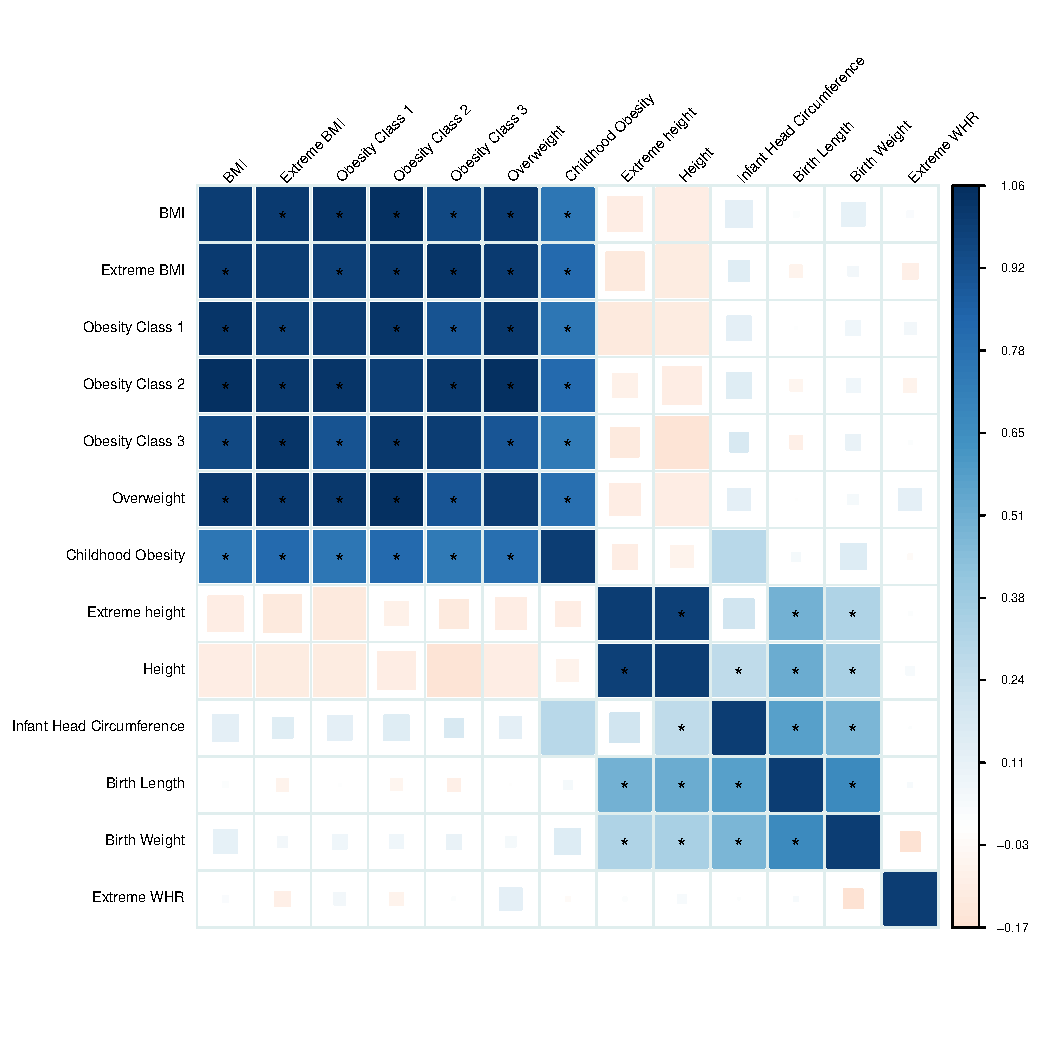
\includegraphics[scale=0.8]{figs/giant_supp.pdf}
\caption{\label{giant}\small{\textit{Genetic correlations among highly correlated anthropometric traits from studies by the GIANT and EGG consortia. The structure of the figure is the same as Figure \ref{Fig:300 Gencors} in the main text: 
blue corresponds to positive genetic correlations; red corresponds to negative genetic correlation. 
Larger squares correspond to more significant $p$-values.
Genetic correlations that are different from zero at 1\% FDR are displayed as full-sized squares. 
Genetic correlations that are significantly different from zero at significance level 0.05 after Bonferroni correction are given an asterisk.}}}
\end{centering}
\end{figure}
\newpage

\subsection*{Genetic Correlations among Smoking Traits}
\begin{figure}[!ht]
\begin{centering}
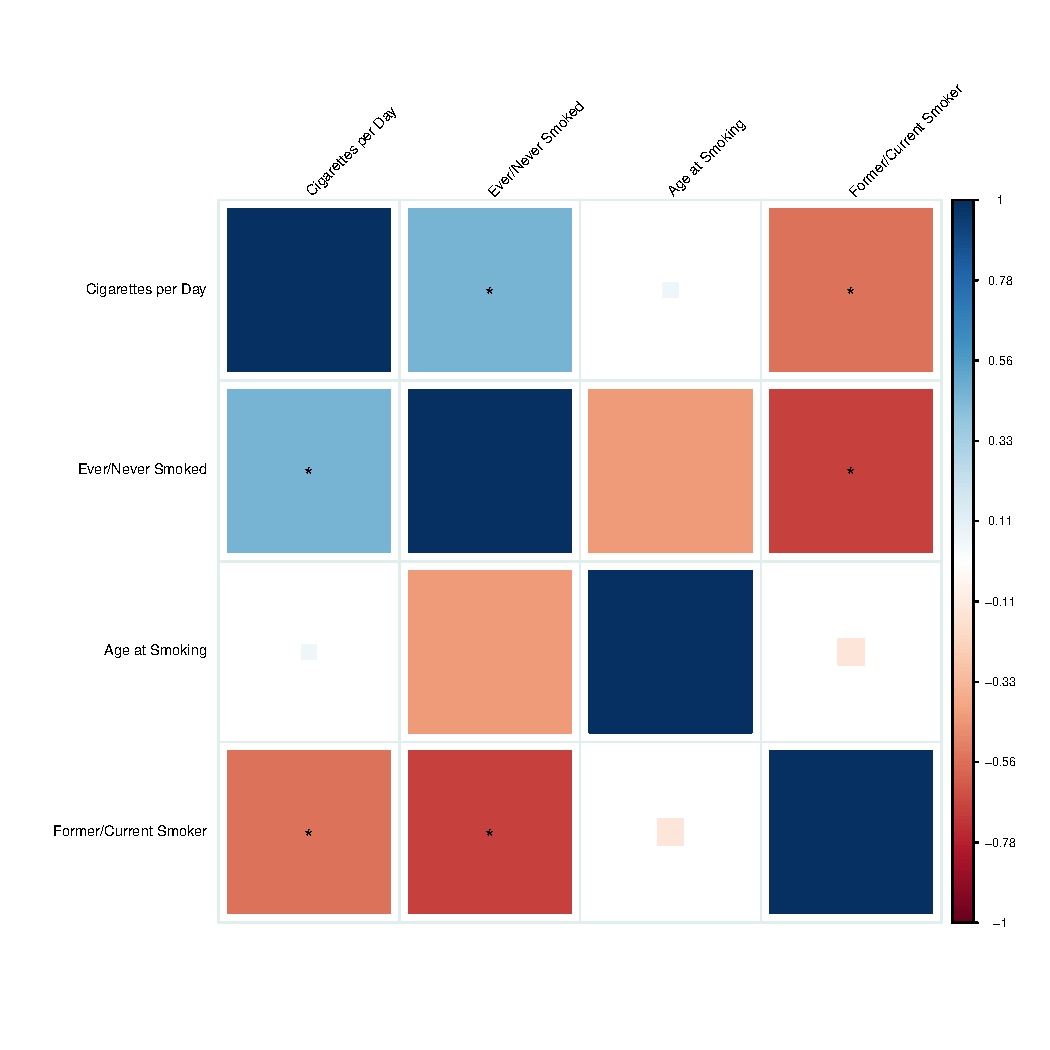
\includegraphics[scale=0.8]{figs/tag_supp.pdf}
\caption{\label{smoking}\small{\textit{Genetic correlations among highly correlated smoking-related traits from the Tobacco and Genetics (TAG) consortium. The structure of the figure is the same as Figure \ref{Fig:300 Gencors} in the main text: 
blue corresponds to positive genetic correlations; red corresponds to negative genetic correlation. 
Larger squares correspond to more significant $p$-values.
Genetic correlations that are different from zero at 1\% FDR are displayed as full-sized squares. 
Genetic correlations that are significantly different from zero at significance level 0.05 after Bonferroni correction are given an asterisk.}}}
\end{centering}
\end{figure}
\newpage

\subsection*{Genetic Correlations among Insulin-Related Traits}
\begin{figure}[!ht]
\begin{centering}
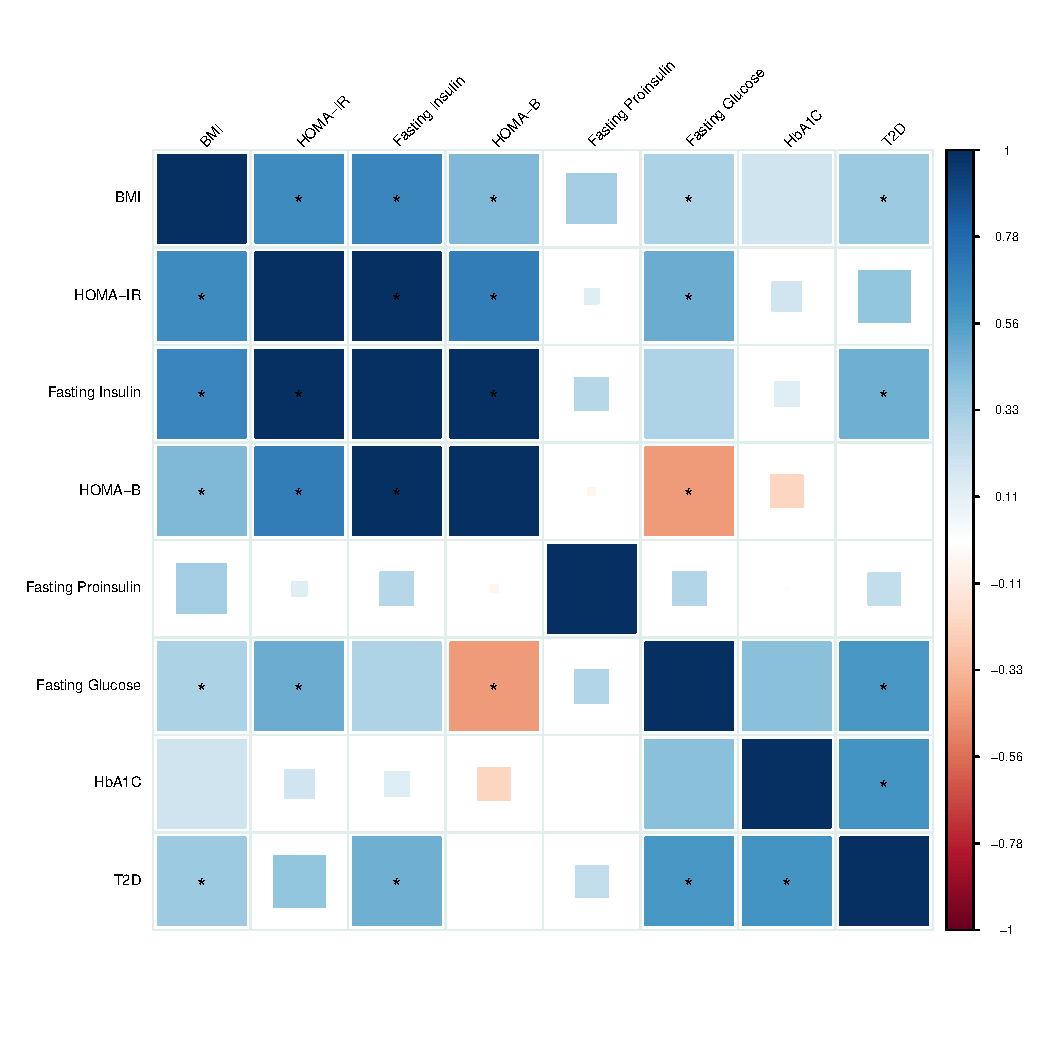
\includegraphics[scale=0.8]{figs/magic_supp.pdf}
\caption{\label{insulin}\small{\textit{Genetic correlations among highly correlated insulin-related traits from studies by the MAGIC consortium. The structure of the figure is the same as Figure \ref{Fig:300 Gencors} in the main text: 
blue corresponds to positive genetic correlations; red corresponds to negative genetic correlation. 
Larger squares correspond to more significant $p$-values.
Genetic correlations that are different from zero at 1\% FDR are displayed as full-sized squares. 
Genetic correlations that are significantly different from zero at significance level 0.05 after Bonferroni correction are given an asterisk.}}}
\end{centering}
\end{figure}
\newpage


\subsection*{Comparison of Metabolic Genetic Correlations from LDSC to Results from Vattikuti, et al}
\begin{figure}[!ht]
\begin{centering}
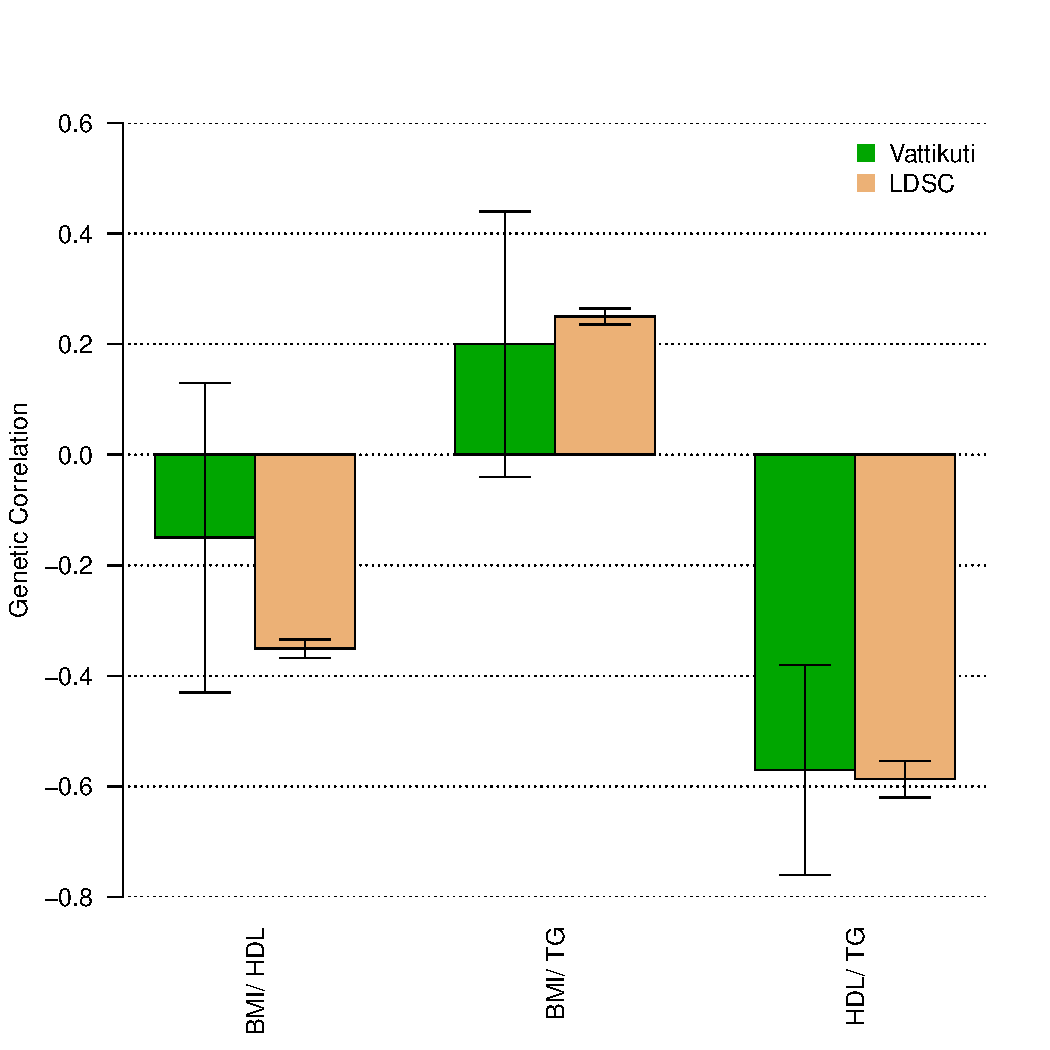
\includegraphics[scale=0.8]{figs/vattikuti.pdf}
\caption{\label{vattikuti}\small{\textit{This figure compares the estimates of genetic correlations between metabolic traits from table 3 of \cite{vattikuti2012heritability}
to the results obtained using roughly 10x larger sample sizes and LD Score regression in this paper.}}}
\end{centering}
\end{figure}
\newpage

\subsection*{Schizophrenia / TG Conditional QQ Plot with and without the MHC}
\begin{figure}[!ht]
\begin{centering}
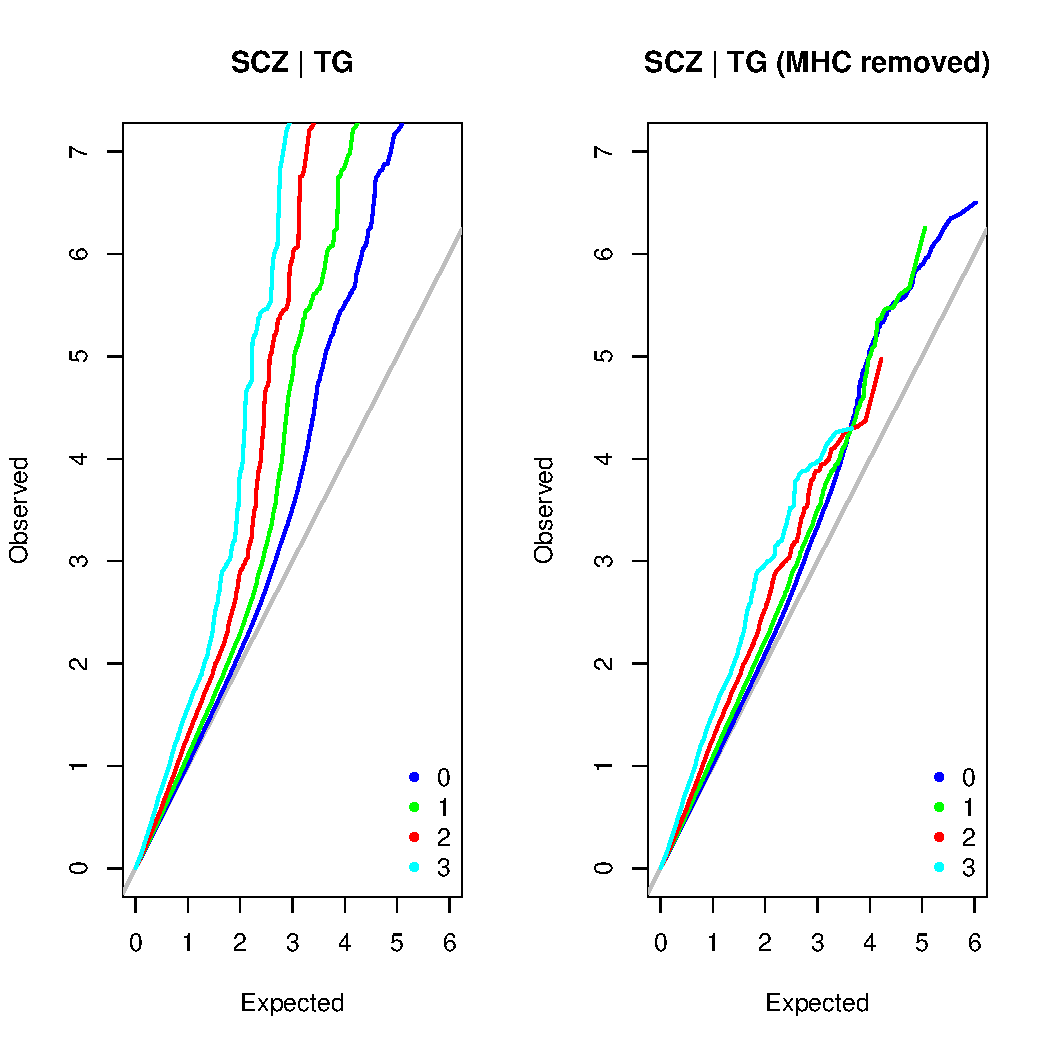
\includegraphics[scale=0.9]{figs/PGC1_pleiotropy_filter.png}
\caption{\label{qq_tg}\small{\textit{We reproduced the conditional QQ plot comparing schizophrenia (SCZ) and triglycerides (TG) from Andreassen et al. \cite{andreassen2013improved} (left). 
The major histocompatibility complex (MHC, approximately chr6, 25-35 MB) is
a genomic region featuring SNPs with exceptionally high LD Scores and the strongest GWAS association to schizophrenia.
Removing the MHC removes almost all signal from the conditional QQ plot (right), which is consistent with the 
near-zero genetic correlation between schizophrenia and TG estimated via LD Score regression.}}}
\end{centering}
\end{figure}
\newpage

%%%%%%%%%%%%%%%%%%%%%%%%%%%%%%%%%%%%%%%%%%%%%%%%%%%%%%%%%%%%%%%
\section*{Collaborators}
%%%%%%%%%%%%%%%%%%%%%%%%%%%%%%%%%%%%%%%%%%%%%%%%%%%%%%%%%%%%%%%


%%%%%%%%%%%%%%%%%%%%%%%%%%%%%%%%%%%%%%%%%%%%%%%%%%%%%%%%%%%%%%%
\section*{Supplementary References}
%%%%%%%%%%%%%%%%%%%%%%%%%%%%%%%%%%%%%%%%%%%%%%%%%%%%%%%%%%%%%%%

\end{document}
